In this section we report the experimental evaluation of OISVMs. As a
simple case-study, we first test the method on a set of databases
commonly used in the machine learning community (section
\ref{exp:ml}); we then apply it to the more realistic scenario of
place recognition, where the aim is to update the model to handle
variations in an indoor environment (section
\ref{exp:idol2}).

OISVMs have been implemented in Matlab and tested against LIBSVM v2.82
\cite{ChangL01}. For the sake of comparison, LIBSVM has been modified
as suggested by the Authors in order to set $p=2$ in
(\ref{eqn:svm_primal}); this modified version is called LIBSVM-2 in
the following.  The software library was also extended to various
families of kernels, and to two approximate incremental extensions of
SVM, the fixed-partition incremental SVM \cite{syed99incremental}, and
the memory-controlled incremental SVM \cite{pronobis:icvs06}.  In the case
of finite-dimensional kernels, we only show the performance of
LIBSVM-2 against OISVMs with $\eta$ at machine precision, since the
solution found by OISVM is \emph{exactly} equivalent; in the case of
infinite-dimensional kernels, we show curves for various values of
$\eta$.

\subsection{Experiments on Standard Benchmark Databases}
\label{exp:ml}

Figure \ref{fig:ad7} and Table \ref{table:t1} show the above mentioned
comparison on some standard benchmark databases\footnote{
\url{http://www.csie.ntu.edu.tw/~cjlin/libsvmtools/datasets}}.  For
each benchmark, data are obtained by running $10$ random $75\%/25\%$
train/test runs.

\begin{figure*}[!ht]
  \centering \footnotesize
  \begin{tabular}{cc}
  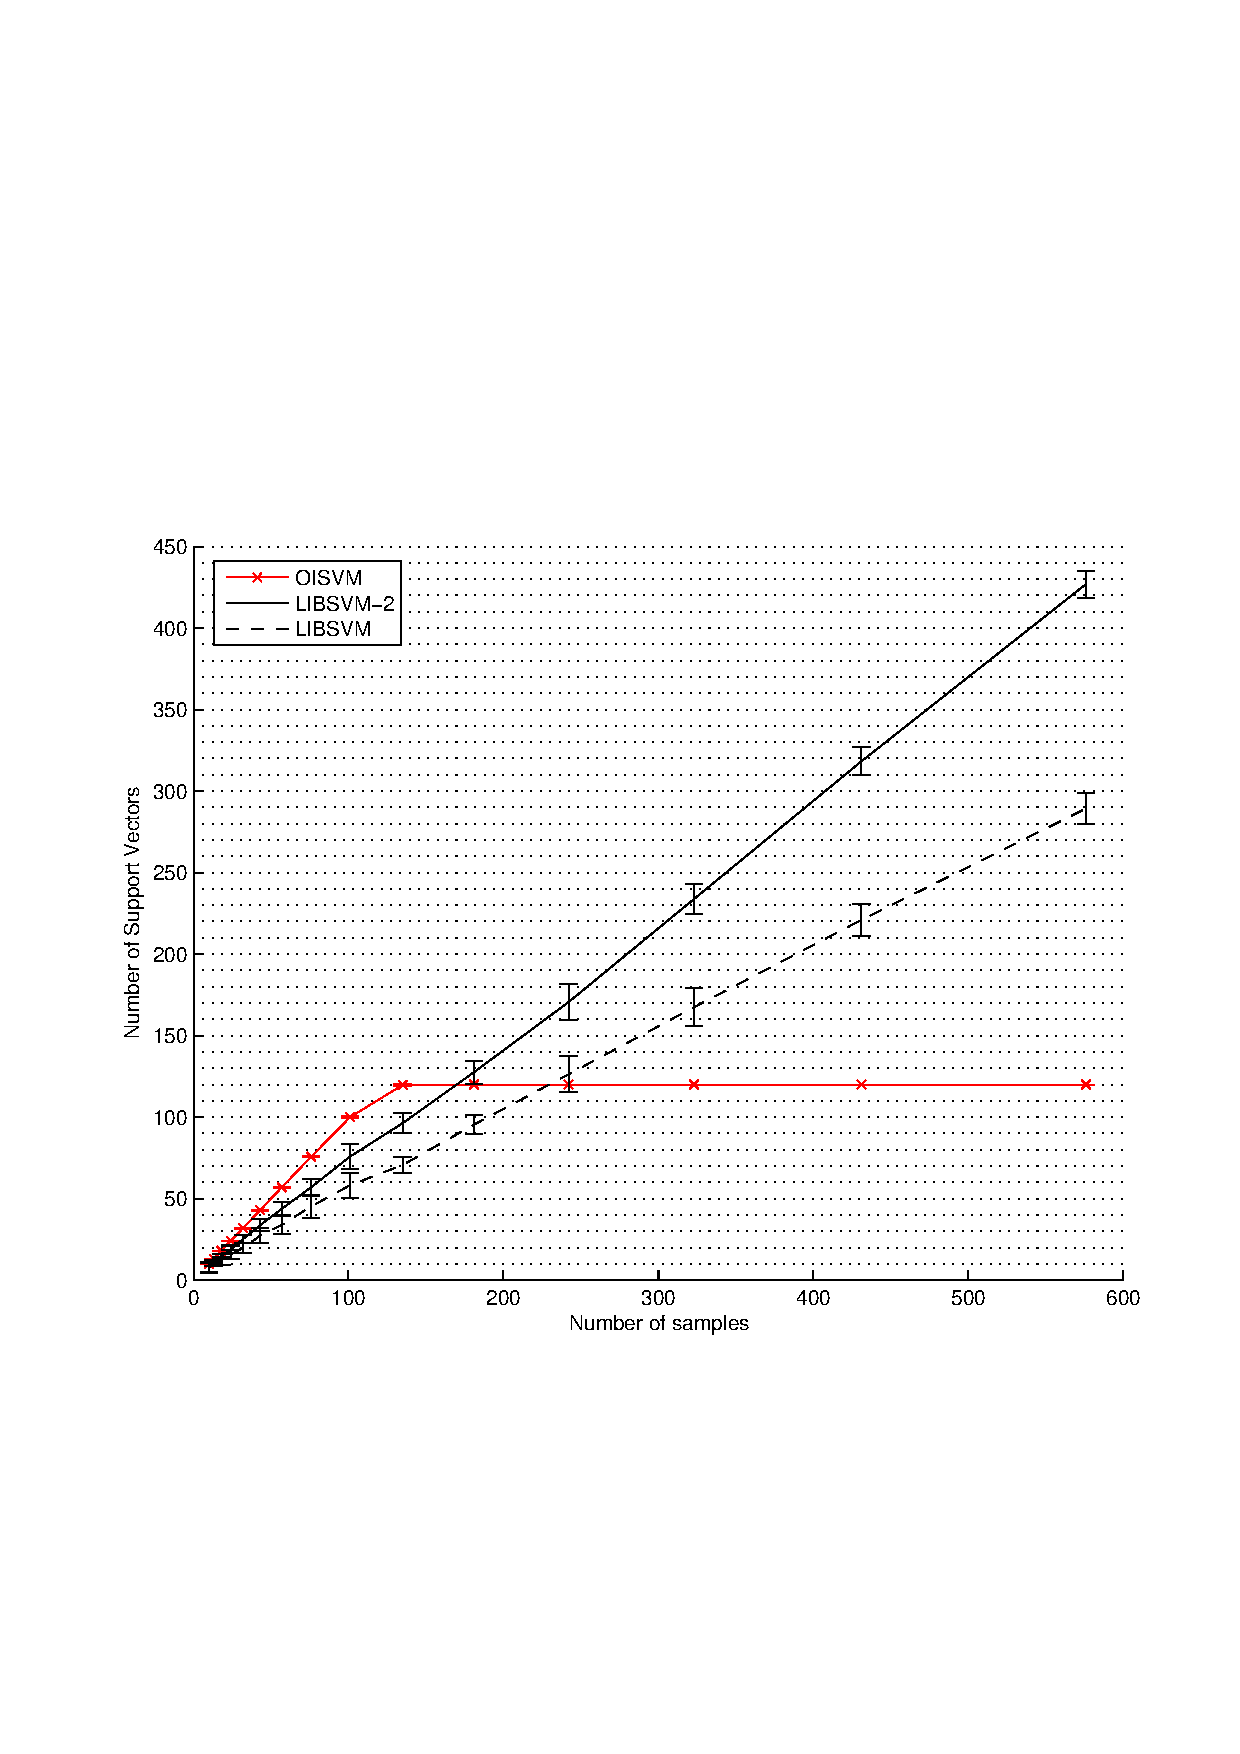
\includegraphics[width=0.47\linewidth]{figs/results/finite_kernel.pdf} &
  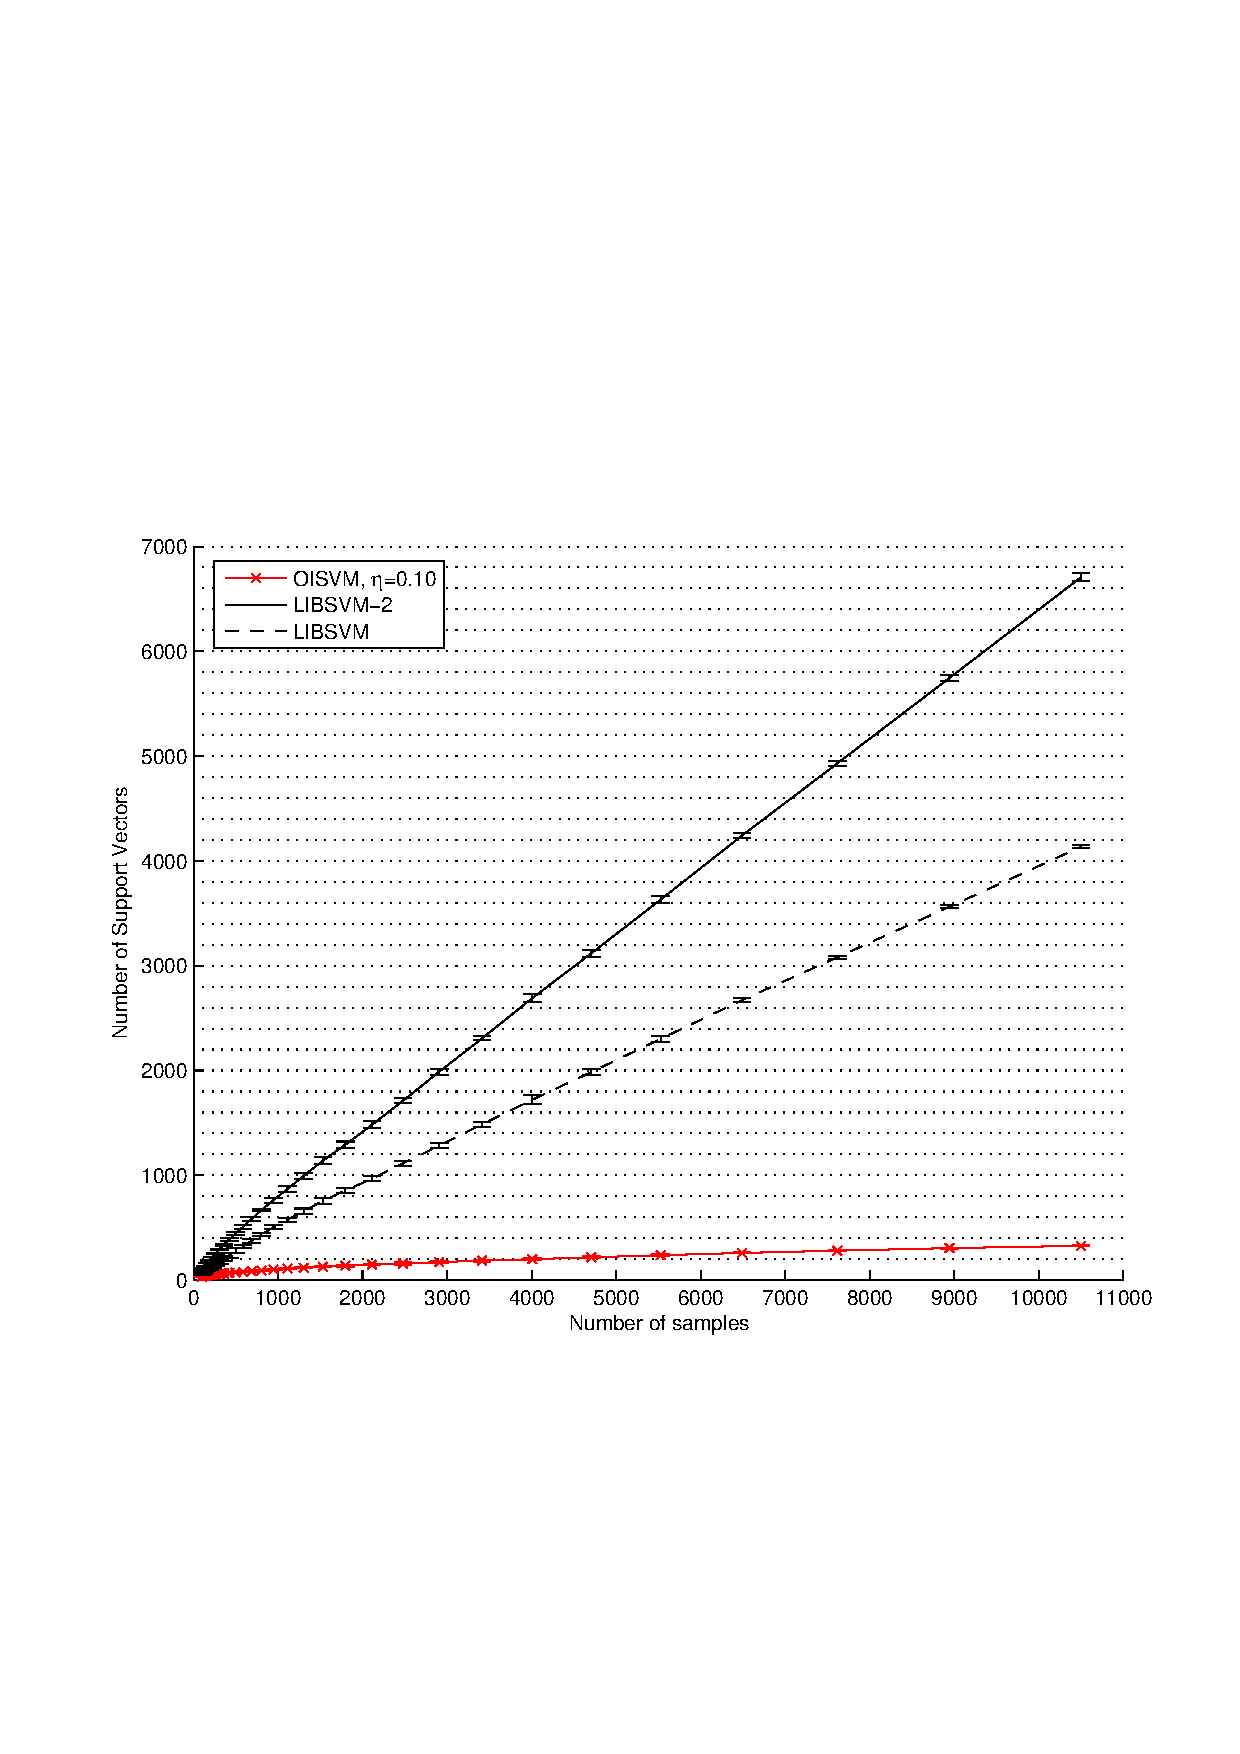
\includegraphics[width=0.47\linewidth]{figs/results/adult7.pdf}
  \end{tabular}
  \caption{Comparison of OISVM and LIBSVM on the \emph{Diabetes}
  (left pane) and \emph{Adult7} (right pane) benchmarks. Diabetes is
  solved using a polynomial kernel with degree $3$, while Adult7 is
  solved using a Gaussian kernel.}
\label{fig:ad7}
\end{figure*}

\begin{table*}
\begin{center}
\begin{tabular}[!h]{|l|c|c|c|}
\hline
  Benchmark & Class. rate    & \% SVs          & \% SVs        \\
       name & loss           & vs. LIBSVM-2    & vs. LIBSVM    \\ \hline
     Breast & $0.47\pm0.82$  & $10.2\pm0.87$   & $22.1\pm1.77$ \\
   Diabetes & $-0.52\pm2.1$  & $40.2\pm2.1$    & $55.2\pm2.73$ \\
   German   & $0.40\pm1.15$  & $6.1\pm0.23$    & $9.2\pm0.35$  \\
   Heart    & $-0.45\pm1.01$ & $10.3\pm0.56$   & $15.5\pm0.94$ \\ \hline
\end{tabular}
\end{center}
\label{table:t1}
\caption{Comparison of OISVM and LIBSVM on more standard benchmarks, solved
 using a Gaussian kernel. For each benchmark, we report the difference
 in classification rate with respect to LIBSVM-2 and the
 percentage of the number of SVs with respect to LIBSVM and
 LIBSVM-2. The value of $\eta$ has been chosen in order not to loose
 more than $0.5\%$ accuracy.}
\end{table*}

Consider Figure \ref{fig:ad7}, left pane: when all samples have been
loaded, LIBSVM-2 has about $427$ SVs, and LIBSVM about $290$. The
kernel used is polynomial with degree $3$ and the benchmark has $8$
features, therefore the dimension of the feature space is
$\binom{10}{3} = 120$ (see, e.g., \cite{Burges98}); and, as expected,
OISVM stops acquiring new SVs when there are exactly $120$, although
it loads a few more before reaching the limit, with respect to the
other approaches. The accuracy (not displayed) is exactly the
same. Again, notice that, after having acquired $120$ SVs, OISVM will
never acquire any more ever, while keeping the same accuracy, whereas
the LIBSVMs do, as theoretically proved in \cite{Steinwart03}.

Consider now Figure \ref{fig:ad7}, right pane: the kernel used is
Gaussian and its dimension is infinite. The benchmark is relevantly
large ($16100$ samples) and complex ($123$ features). Nevertheless,
with an $\eta$ as small as $0.1$, at the end OISVM has less than $5\%$
of the SVs used by LIBSVM-2 and less than $8\%$ with respect to
LIBSVM. The accuracy is $0.063\%\pm0.14$ worse than that of LIBSVM-2.

Lastly, consider Table \ref{table:t1}, which shows the very same data
in compact form for $4$ more standard databases. OISVM attains a
number of SVs which is about $6\%$ to slightly more than $55\%$ of
LIBSVM, whereas the accuracy is basically the same, being slightly
better than LIBSVM in two cases (\emph{Diabetes}, this time solved via
a Gaussian kernel, and \emph{Heart}).
